%author : berenice delcroix-oger

\documentclass[border=2pt]{standalone}
\usepackage{tikz}
\usetikzlibrary{positioning, fit, shapes, arrows, calc}

\pgfdeclarelayer{bg}    % declare background layer
\pgfsetlayers{bg,main}  % set the order of the layers (main is the standard layer)

\newcommand{\coula}{0785F2}
\newcommand{\coulb}{F29F05}
\newcommand{\coulc}{F21313}
\newcommand{\could}{E6F21F}



\definecolor{part1}{HTML}{\coula}
\definecolor{part2}{HTML}{\coulb}
\definecolor{part3}{HTML}{\coulc}
\definecolor{part4}{HTML}{\could}

\begin{document}
\begin{tikzpicture}
\node (min) at (0,0){
\begin{tikzpicture}[scale=0.3, inner sep=1pt]
\node[draw, circle] (1p){1};
\node[draw, circle, right=5pt of 1p](3p){2};
\node[draw, circle, right=5pt of 3p](2p){3};
\end{tikzpicture}};
\node[above left=1cm of min.north] (3) {
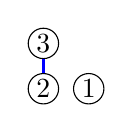
\begin{tikzpicture}[scale=0.3, inner sep=1pt]
\node[draw, circle] (1p){2};
\node[draw, circle, above=5pt of 1p](3p){3};
\node[draw, circle, right=5pt of 1p](2p){1};
\draw[very thick, blue] (1p)--(3p);
\end{tikzpicture}};
\node[above right=1cm of min.north] (4) {
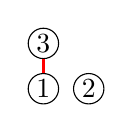
\begin{tikzpicture}[scale=0.3, inner sep=1pt]
\node[draw, circle] (1p){1};
\node[draw, circle, above=5pt of 1p](3p){3};
\node[draw, circle, right=5pt of 1p](2p){2};
\draw[very thick, red] (1p)--(3p);
\end{tikzpicture}};
\node[left=0.5cm of 3] (2) {
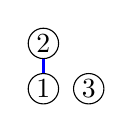
\begin{tikzpicture}[scale=0.3, inner sep=1pt]
\node[draw, circle] (1p){1};
\node[draw, circle, above=5pt of 1p](3p){2};
\node[draw, circle, right=5pt of 1p](2p){3};
\draw[very thick, blue] (1p)--(3p);
\end{tikzpicture}};
\node[left=0.5cm of 2] (1) {
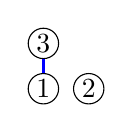
\begin{tikzpicture}[scale=0.3, inner sep=1pt]
\node[draw, circle] (1p){1};
\node[draw, circle, above=5pt of 1p](3p){3};
\node[draw, circle, right=5pt of 1p](2p){2};
\draw[very thick, blue] (1p)--(3p);
\end{tikzpicture}};
\node[right=0.5cm of 4] (5) {
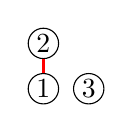
\begin{tikzpicture}[scale=0.3, inner sep=1pt]
\node[draw, circle] (1p){1};
\node[draw, circle, above=5pt of 1p](3p){2};
\node[draw, circle, right=5pt of 1p](2p){3};
\draw[very thick, red] (1p)--(3p);
\end{tikzpicture}};
\node[right=0.5cm of 5] (6) {
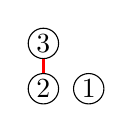
\begin{tikzpicture}[scale=0.3, inner sep=1pt]
\node[draw, circle] (1p){2};
\node[draw, circle, above=5pt of 1p](3p){3};
\node[draw, circle, right=5pt of 1p](2p){1};
\draw[very thick, red] (1p)--(3p);
\end{tikzpicture}};
\node[above=2cm of 1] (15) {
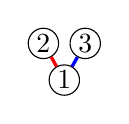
\begin{tikzpicture}[scale=0.3, inner sep=1pt]
\node[draw, circle] (1p){1};
\node[draw, circle, above left=5pt of 1p.north](2p){2};
\node[draw, circle, above right=5pt of 1p.north](3p){3};
\draw[very thick, blue] (1p)--(3p);
\draw[very thick, red] (1p)--(2p);
\end{tikzpicture}};
\node[left=0.5cm of 15] (123) {
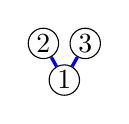
\begin{tikzpicture}[scale=0.3, inner sep=1pt]
\node[draw, circle] (1p){1};
\node[draw, circle, above left=5pt of 1p.north](2p){2};
\node[draw, circle, above right=5pt of 1p.north](3p){3};
\draw[very thick, blue] (1p)--(3p);
\draw[very thick, blue] (1p)--(2p);
\end{tikzpicture}};
\node[right=0.5cm of 15] (26) {
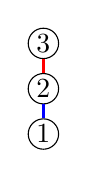
\begin{tikzpicture}[scale=0.3, inner sep=1pt]
\node[draw, circle] (1p){1};
\node[draw, circle, above=5pt of 1p.north](2p){2};
\node[draw, circle, above=5pt of 2p.north](3p){3};
\draw[very thick, red] (2p)--(3p);
\draw[very thick, blue] (1p)--(2p);
\end{tikzpicture}};
\node[right=0.5cm of 26] (34) {
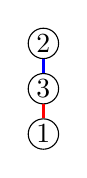
\begin{tikzpicture}[scale=0.3, inner sep=1pt]
\node[draw, circle] (1p){1};
\node[draw, circle, above=5pt of 1p.north](2p){3};
\node[draw, circle, above=5pt of 2p.north](3p){2};
\draw[very thick, blue] (2p)--(3p);
\draw[very thick, red] (1p)--(2p);
\end{tikzpicture}};
\node[right=0.5cm of 34] (24) {
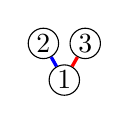
\begin{tikzpicture}[scale=0.3, inner sep=1pt]
\node[draw, circle] (1p){1};
\node[draw, circle, above left=5pt of 1p.north](2p){2};
\node[draw, circle, above right=5pt of 1p.north](3p){3};
\draw[very thick, red] (1p)--(3p);
\draw[very thick, blue] (1p)--(2p);
\end{tikzpicture}};
\node[right=0.5cm of 24] (35) {
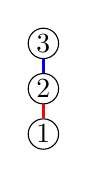
\begin{tikzpicture}[scale=0.3, inner sep=1pt]
\node[draw, circle] (1p){1};
\node[draw, circle, above=5pt of 1p.north](2p){2};
\node[draw, circle, above=5pt of 2p.north](3p){3};
\draw[very thick, blue] (2p)--(3p);
\draw[very thick, red] (1p)--(2p);
\end{tikzpicture}};
\node[right=0.5cm of 35] (16) {
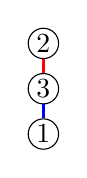
\begin{tikzpicture}[scale=0.3, inner sep=1pt]
\node[draw, circle] (1p){1};
\node[draw, circle, above=5pt of 1p.north](2p){3};
\node[draw, circle, above=5pt of 2p.north](3p){2};
\draw[very thick, red] (2p)--(3p);
\draw[very thick, blue] (1p)--(2p);
\end{tikzpicture}};
\node[right=0.5cm of 16] (456) {
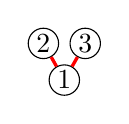
\begin{tikzpicture}[scale=0.3, inner sep=1pt]
\node[draw, circle] (1p){1};
\node[draw, circle, above left=5pt of 1p.north](2p){2};
\node[draw, circle, above right=5pt of 1p.north](3p){3};
\draw[very thick, red] (1p)--(3p);
\draw[very thick, red] (1p)--(2p);
\end{tikzpicture}};
\draw (min)--(1);
\draw (min)--(2);
\draw (min)--(3);
\draw (min)--(4);
\draw (min)--(5);
\draw (min)--(6);
\draw (123.south)--(1.north);
\draw (123.south)--(2.north);
\draw (123.south)--(3.north);
\draw (456.south)--(4.north);
\draw (456.south)--(5.north);
\draw (456.south)--(6.north);
\draw (2.north)--(26.south)--(6.north);
\draw (2.north)--(24.south)--(4.north);
\draw (1.north)--(15.south)--(5.north);
\draw (1.north)--(16.south)--(6.north);
\draw (3.north)--(34.south)--(4.north);
\draw (3.north)--(35.south)--(5.north);
\end{tikzpicture}

\end{document}
